\documentclass{article}
\usepackage{listings}
\usepackage{graphicx} % Required for inserting images
\usepackage{color}
\usepackage[a4paper, total={6.5in, 10in}]{geometry}
\usepackage{enumitem}

\lstnewenvironment{C}
  {\lstset{language=C}} 
%Add your addition parameters as required like showstringspaces , line numbering , 
% frames , etc.seperated by a comma as shown in the CPP  environment 
  {}
\lstnewenvironment{CPP}
  {\lstset{language=C++,basicstyle=\ttfamily\small,frame=none}}
  {}
\lstnewenvironment{Java}
  {\lstset{language=Java}}
  {}
\lstnewenvironment{Python}
  {\lstset{language=Python}}
  {}

% \title{\huge TP3 Report \\ Artificial Intelligence}
% \author{Bruno Luiz Dias Alves de Castro \\ Victor Gabriel Mendes Sündermann}
% \date{April 2023}

\begin{document}
\definecolor{light-gray}{gray}{0.95}

\begin{titlepage}
\centering
{\textsc{\Large ESIEE Paris \\ ~\\ Artificial Intelligence and Cybersecurity} \par}
\vfill
{\huge\bfseries Artificial Intelligence \par}
\vspace{0.5cm}
{\LARGE Lab 4 Report \par}
\vspace{2cm}
{\Large\itshape Antoine Debauge \par}
{\Large\itshape Bruno Luiz Dias Alves de Castro \par}
{\Large\itshape Victor Gabriel Mendes Sündermann \par}
\vfill

% Bottom of the page
{\large \today\par}
\end{titlepage}

\pagebreak
\tableofcontents
\pagebreak

\section{Introduction}

In this report we will present the results of the fourth project of the Artificial Intelligence course. The project consists of implementing reinforcement learning algorithms and agents to score actions on a grid and eventually solve the \textbf{Pacman} game.
The topics worked on this lab were: Value Iteration, Q-Learning, and aproximate Q-Learning.

\section{Value Iteration}
The code implemented for this algorithm can be seen in Tables~\ref{tab:runValueIteration},~\ref{tab:computeQValueFromValues},~and~\ref{tab:computeActionFromValues}.

\hbox{}

\begin{table} [ht!]
\begin{lstlisting}[language=python, frame=tlbr, framesep=6pt, backgroundcolor=\color{light-gray}]
def runValueIteration(self):
  """
    Run the value iteration algorithm. Note that in standard
    value iteration, V_k+1(...) depends on V_k(...)'s.
  """

  for i in range(self.iterations):
      values = self.values.copy()
      for state in self.mdp.getStates():
          if self.mdp.isTerminal(state):
              continue
              
          max_value = float("-inf")
          for action in self.mdp.getPossibleActions(state):
              max_value = \ 
                max(max_value, self.computeQValueFromValues(state, action))
          values[state] = max_value
      self.values = values
\end{lstlisting}
\caption{runValueIteration function}
\label{tab:runValueIteration}
\end{table}

\begin{table} [ht!]
\begin{lstlisting}[language=python, frame=tlbr, framesep=6pt, backgroundcolor=\color{light-gray}]
def computeQValueFromValues(self, state, action):
  """
    Compute the Q-value of action in state from the
    value function stored in self.values.
  """

  q_value = 0
  for next_state, prob in self.mdp.getTransitionStatesAndProbs(state, action):
      q_value += prob * (self.mdp.getReward(state, action, next_state) \ 
      + self.discount * self.values[next_state])

  return q_value
\end{lstlisting}
\caption{computeQValueFromValues function}
\label{tab:computeQValueFromValues}
\end{table}

\begin{table} [ht!]
\begin{lstlisting}[language=python, frame=tlbr, framesep=6pt, backgroundcolor=\color{light-gray}]
def computeActionFromValues(self, state):
  """
    The policy is the best action in the given state
    according to the values currently stored in self.values.

    You may break ties any way you see fit.  Note that if
    there are no legal actions, which is the case at the
    terminal state, you should return None.
  """
  
  if self.mdp.isTerminal(state):
      return None

  max_value = float("-inf")
  best_action = None
  for action in self.mdp.getPossibleActions(state):
      q_value = self.computeQValueFromValues(state, action)
      if q_value > max_value:
          max_value = q_value
          best_action = action

  return best_action
\end{lstlisting}
\caption{computeActionFromValues function}
\label{tab:computeActionFromValues}
\end{table}
  
To run the program, we use the following command:

\hbox{}
  
\begin{lstlisting}[language=bash, frame=tlbr, framesep=6pt, backgroundcolor=\color{light-gray}]
  python3 gridworld.py -a value -i 5
\end{lstlisting}

\hbox{}

This test created the expected output as shown in the following image:

\begin{table}[ht!]
  \begin{center}
    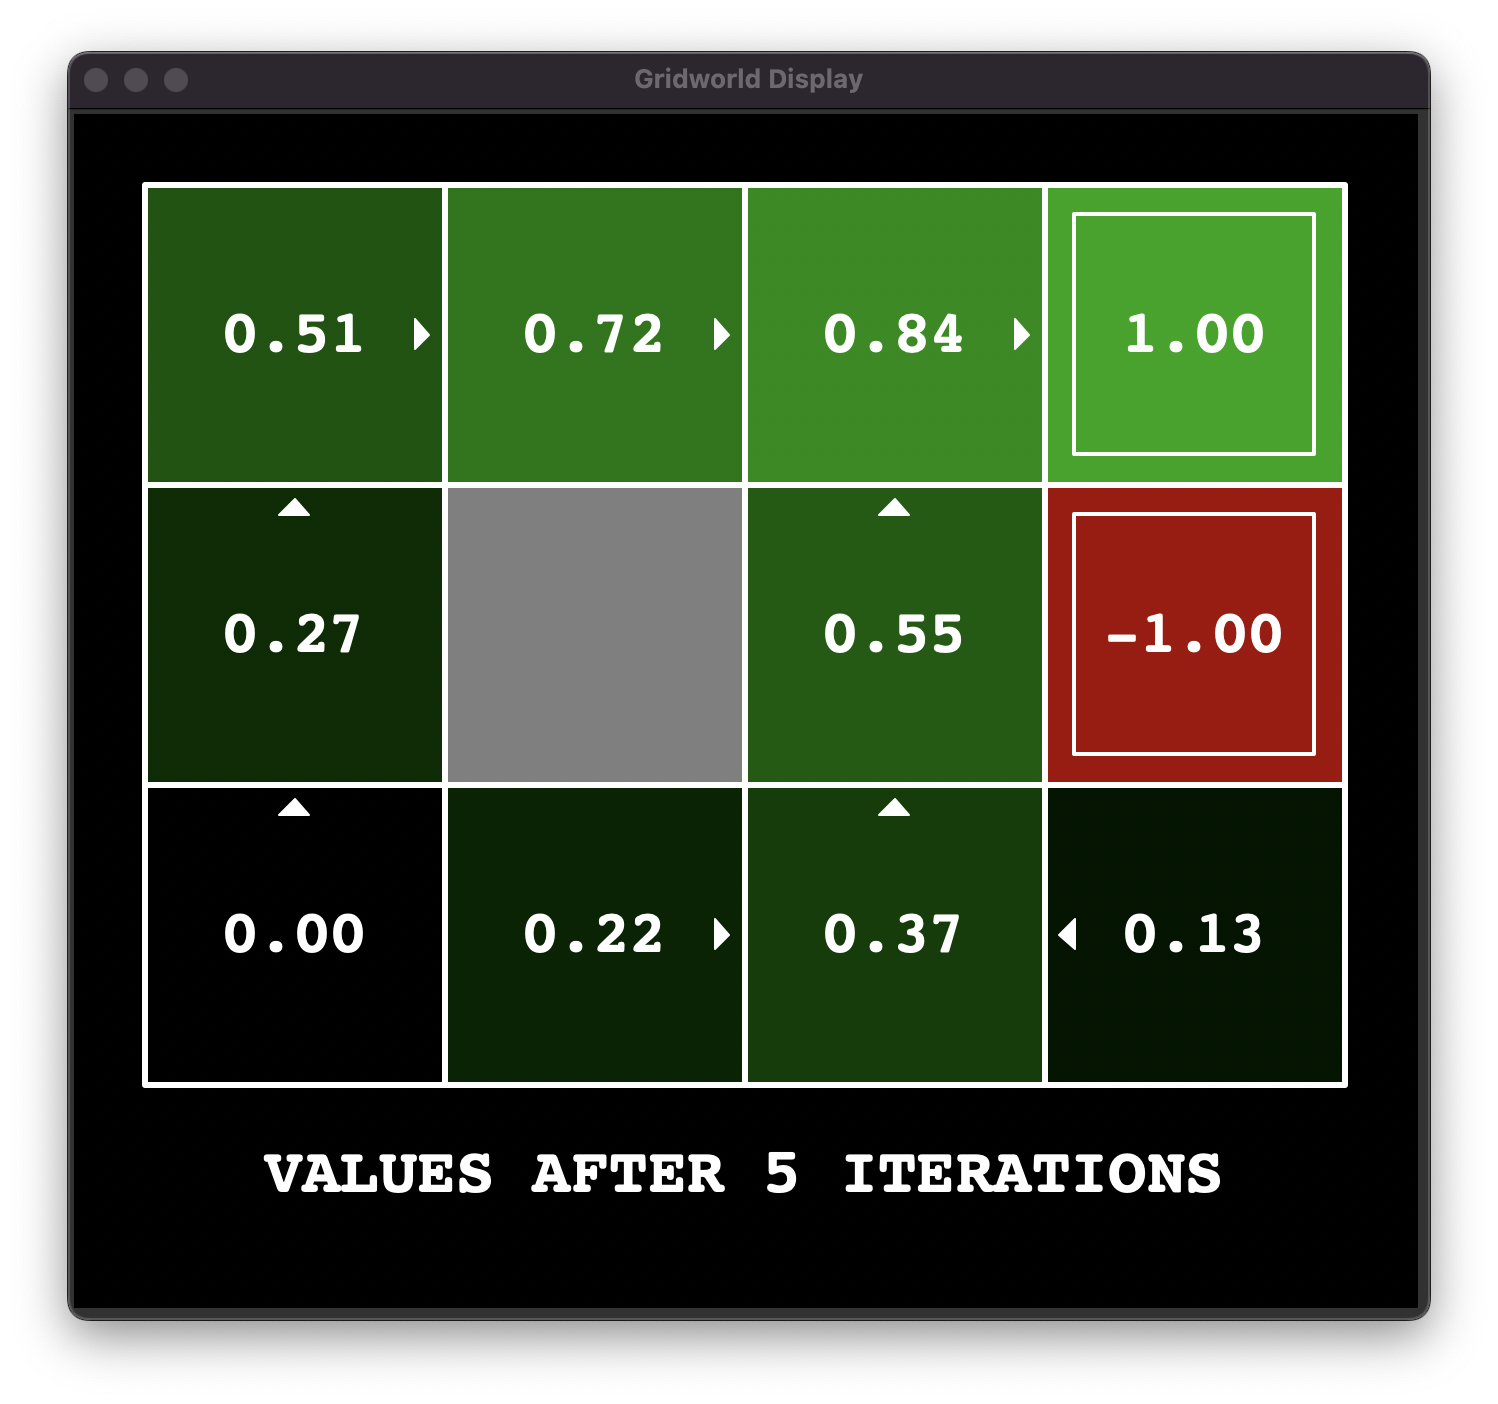
\includegraphics[width=0.5\textwidth]{images/gridWorld-ex2.png}
  \end{center}
\caption{GridWorld with Value Iteration}
\end{table}

Then we tested the code in a bigger scale and executing the policies more times, with the command:

\definecolor{light-gray}{gray}{0.95}
\begin{lstlisting}[language=bash, frame=tlbr, framesep=6pt, backgroundcolor=\color{light-gray}]
  python3 gridworld.py -a value -i 100 -k 10
\end{lstlisting}

The result can be seen bellow:

\begin{table}[ht!]
  \begin{center}
    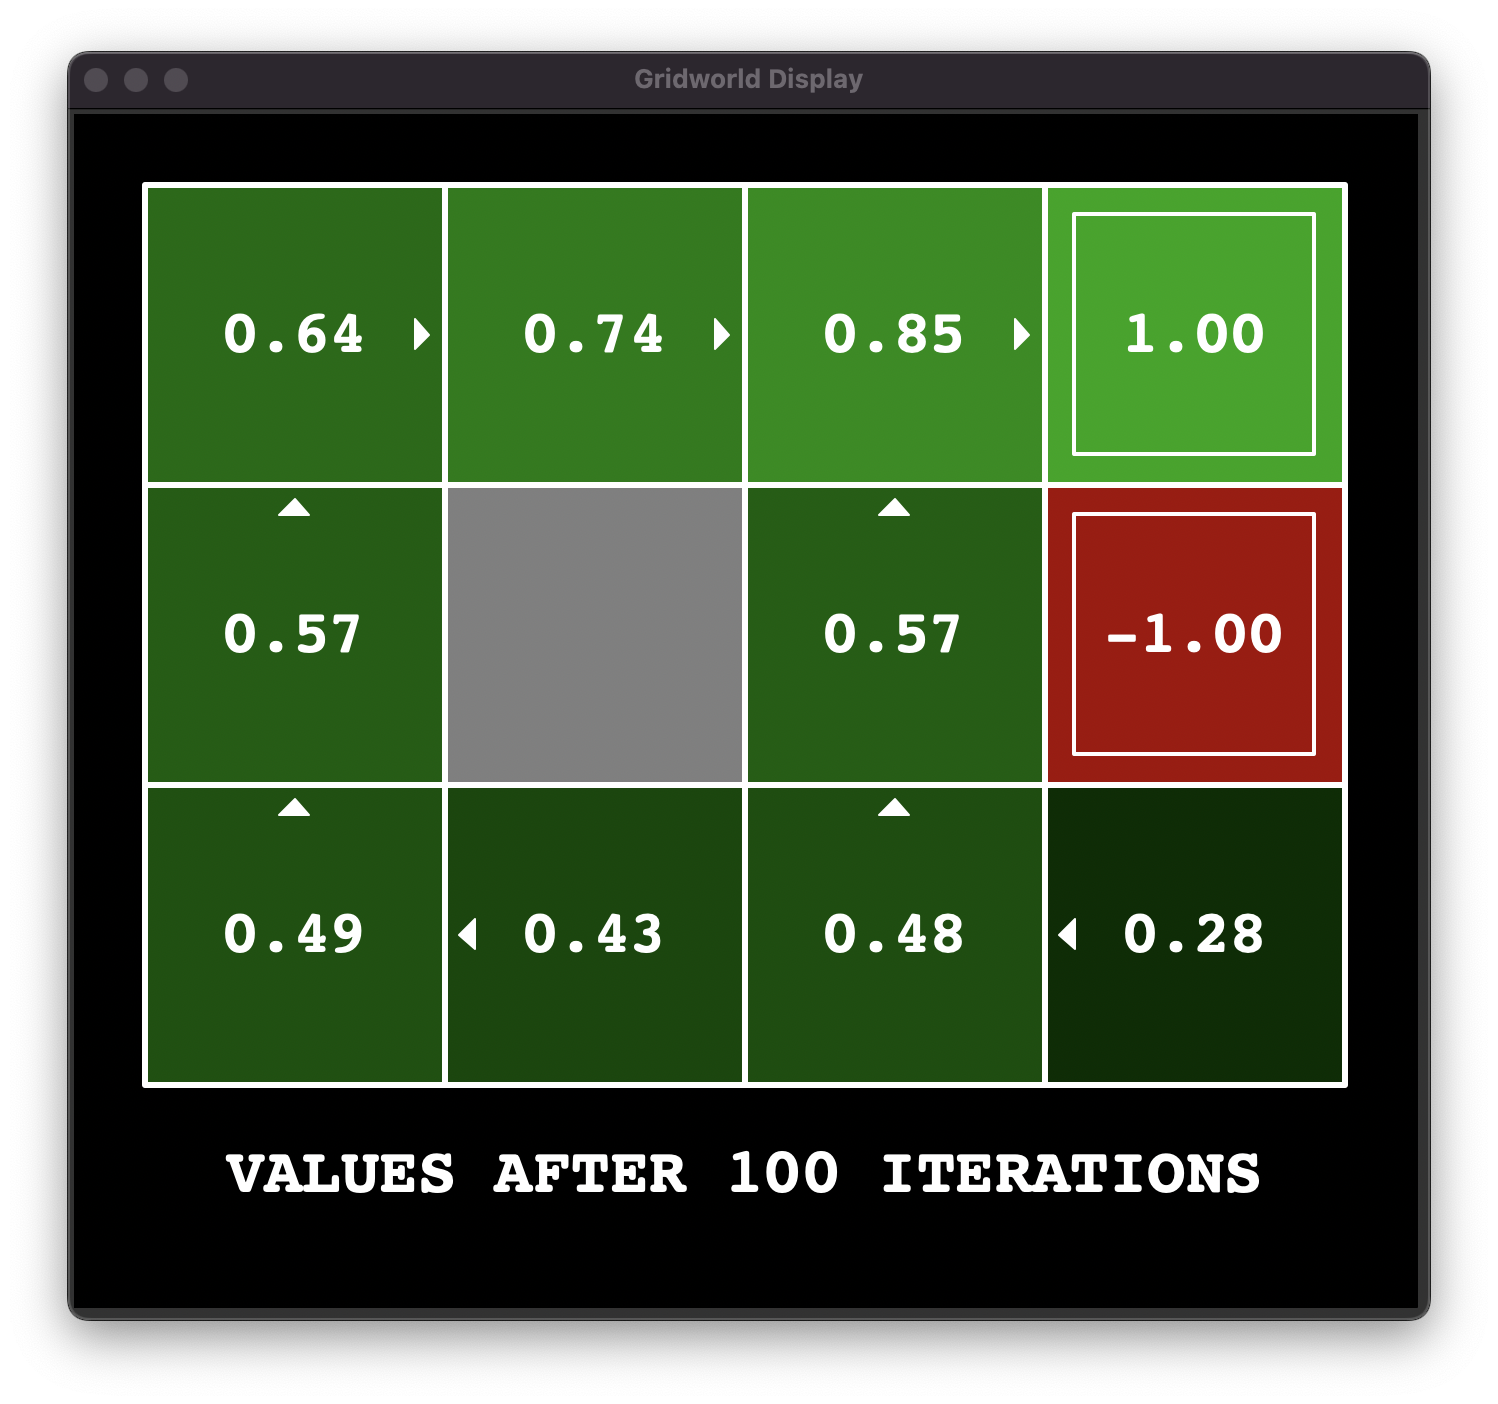
\includegraphics[width=0.5\textwidth]{images/gridWorld-ex3.png}
  \end{center}
\caption{GridWorld with Value Iteration k=100}
\end{table}

\begin{table}[ht!]
  \begin{center}
    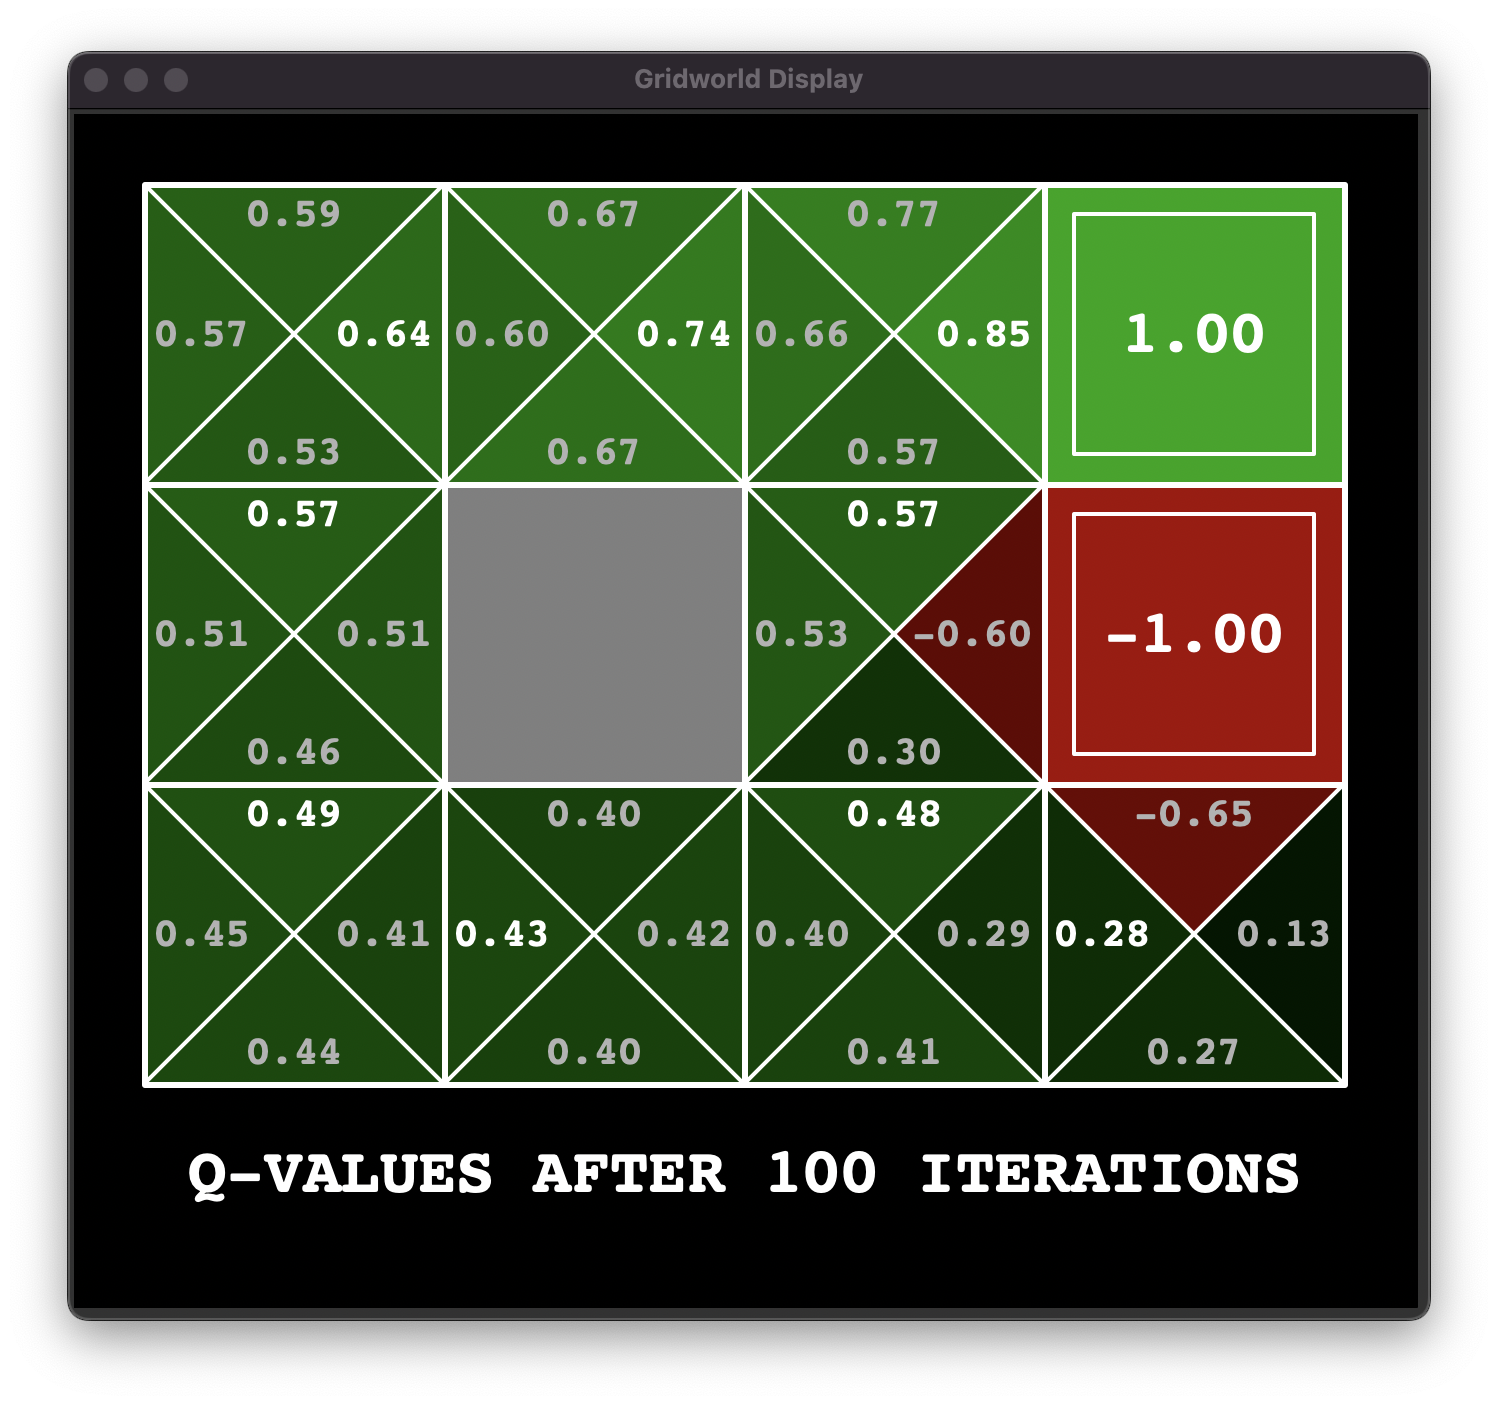
\includegraphics[width=0.5\textwidth]{images/qValues-ex3.png}
  \end{center}
\caption{Q-Values after 100 iterations}
\end{table}

\pagebreak
\section{Q-Learning}

The objective of this section is implementing a Q-Learning agent that learns through trial and error, this agent is constitued of five functions: init(), update(), computeValuefromQValues(), getQValue() and computeActionFromQValues().
The implementation of each of those functions can be seen bellow:

\begin{table} [ht!]
  \begin{lstlisting}[language=python, frame=tlbr, framesep=6pt, backgroundcolor=\color{light-gray}]
  def __init__(self, **args):
  "You can initialize Q-values here..."
  ReinforcementAgent.__init__(self, **args)

  # Q-values
  self.qValuesDict = {}
  \end{lstlisting}
  \caption{init function}
\end{table}

\begin{table} [ht!]
  \begin{lstlisting}[language=python, frame=tlbr, framesep=6pt, backgroundcolor=\color{light-gray}]
  def update(self, state, action, nextState, reward: float):
  """
    The parent class calls this to observe a
    state = action => nextState and reward transition.
    You should do your Q-Value update here
    NOTE: You should never call this function,
    it will be called on your behalf
  """
  
  # Compute sample
  sample = reward + self.discount * self.computeValueFromQValues(nextState)

  # Update Q-value
  self.qValuesDict[(state, action)] = (1 - self.alpha) * \
    self.getQValue(state, action) + self.alpha * sample

  \end{lstlisting}
  \caption{update function}
\end{table}

\begin{table} [ht!]
  \begin{lstlisting}[language=python, frame=tlbr, framesep=6pt, backgroundcolor=\color{light-gray}]
  def computeValueFromQValues(self, state):
  """
    Returns max_action Q(state,action)
    where the max is over legal actions.  Note that if
    there are no legal actions, which is the case at the
    terminal state, you should return a value of 0.0.
  """
  
  legalActions = self.getLegalActions(state)
  if len(legalActions) == 0:
      return 0.0

  maxQValue = -math.inf
  for action in legalActions:
      qValue = self.getQValue(state, action)
      if qValue > maxQValue:
          maxQValue = qValue

  return maxQValue
  \end{lstlisting}
  \caption{computeValuefromQValues function}
\end{table}

\begin{table} [ht!]
  \begin{lstlisting}[language=python, frame=tlbr, framesep=6pt, backgroundcolor=\color{light-gray}]
  def getQValue(self, state, action):
  """
    Returns Q(state,action)
    Should return 0.0 if we have never seen a state
    or the Q node value otherwise
  """
  if (state, action) not in self.qValuesDict:
      self.qValuesDict[(state, action)] = 0.0

  return self.qValuesDict[(state, action)]
  \end{lstlisting}
  \caption{getQValue function}
\end{table}

\begin{table} [ht!]
  \begin{lstlisting}[language=python, frame=tlbr, framesep=6pt, backgroundcolor=\color{light-gray}]
  def computeActionFromQValues(self, state):
  """
    Compute the best action to take in a state.  Note that if there
    are no legal actions, which is the case at the terminal state,
    you should return None.
  """
  
  legalActions = self.getLegalActions(state)
  if len(legalActions) == 0:
      return None

  maxQValue = -math.inf
  bestAction = None
  for action in legalActions:
      qValue = self.getQValue(state, action)
      if qValue > maxQValue:
          maxQValue = qValue
          bestAction = action

  return bestAction
  \end{lstlisting}
  \caption{computeActionFromQValues function}
\end{table}

Now that the Q-Learning agent is done it's time to test it with the following command:

\definecolor{light-gray}{gray}{0.95}
\begin{lstlisting}[language=bash, frame=tlbr, framesep=6pt, backgroundcolor=\color{light-gray}]
  python3 gridworld.py -a q -k 5 -m
\end{lstlisting}

We controlled the agent manually throught the grid and achieved the following result:

\begin{table}[ht!]
  \begin{center}
    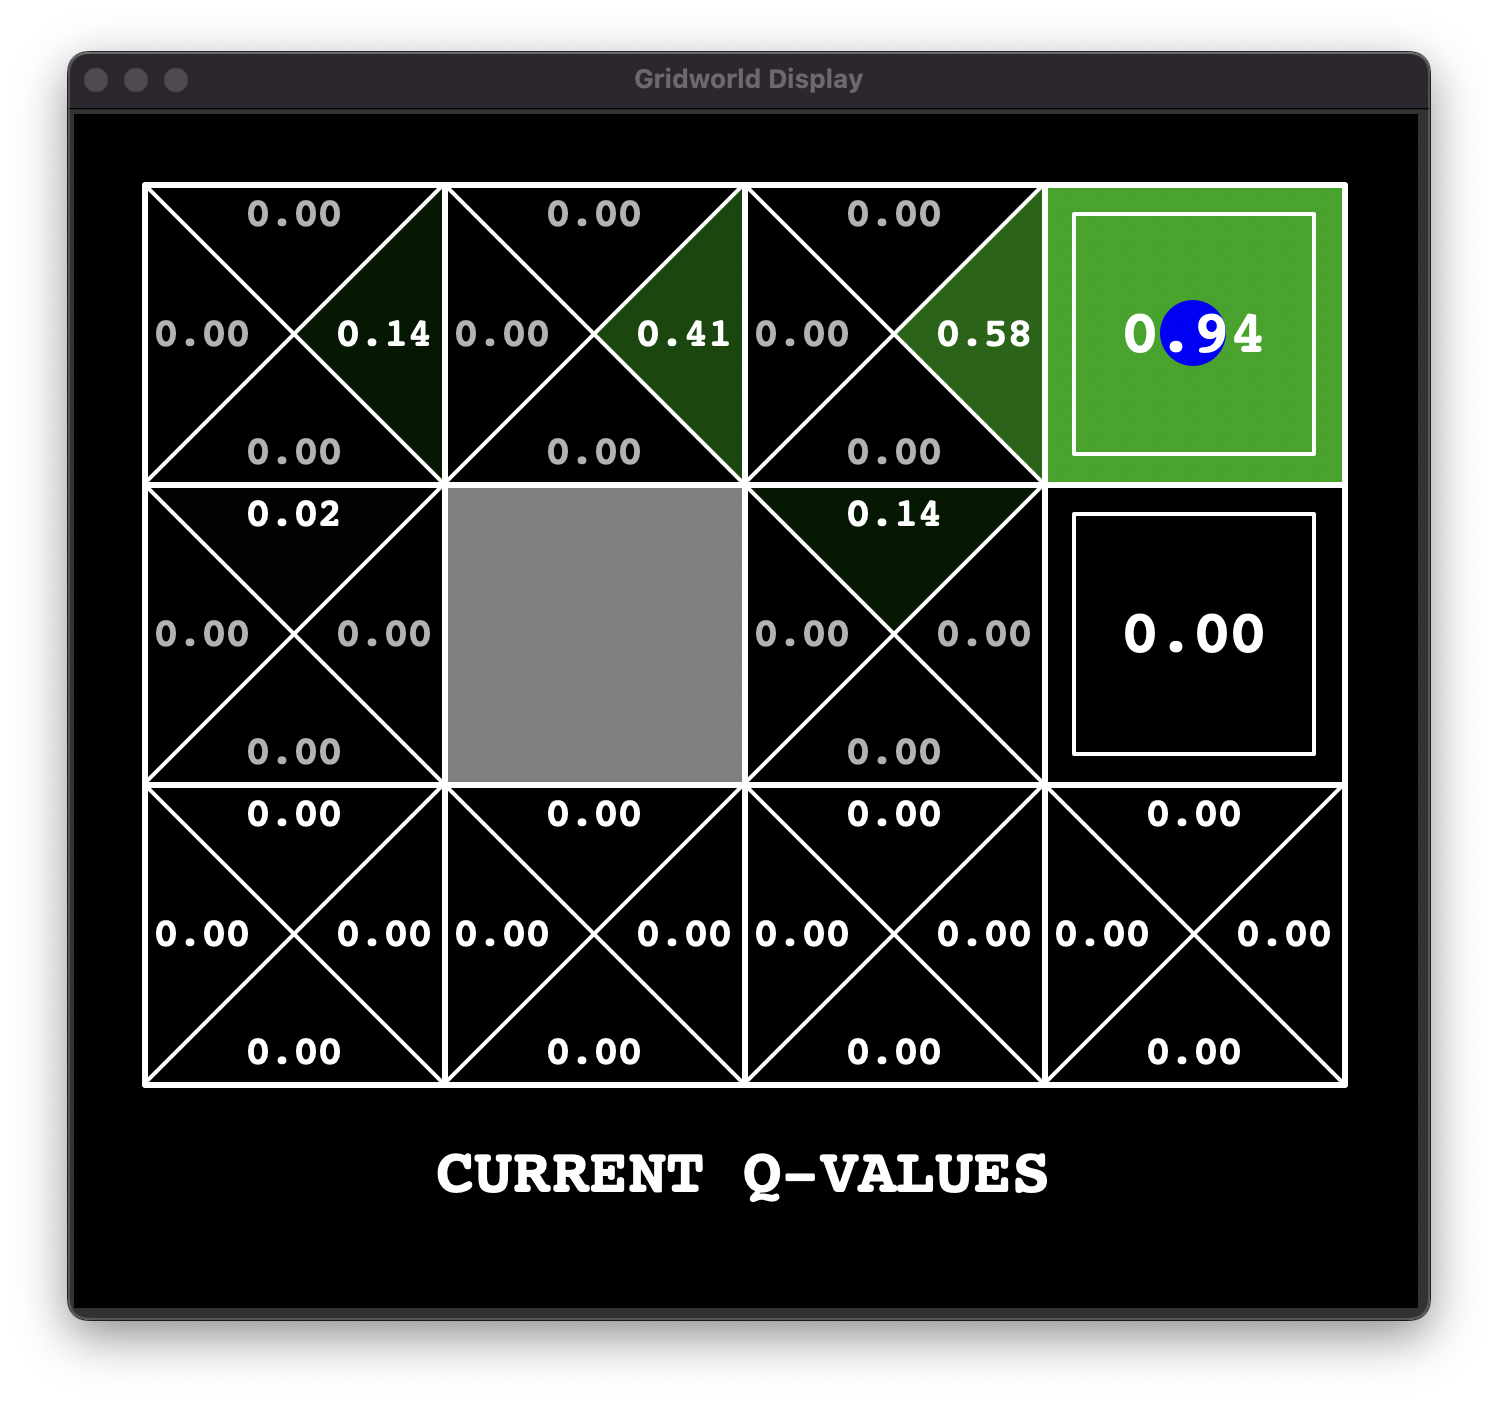
\includegraphics[width=0.5\textwidth]{images/qLearning-ex2.png}
  \end{center}
\caption{Q-Learning agent with manual iteration}
\end{table}

Now we'll add the episilon-greedy cut to automate our agent and see how it performs, for this we ran the following command, which executes the agent 100 times:

\hbox{}
\definecolor{light-gray}{gray}{0.95}
\begin{lstlisting}[language=bash, frame=tlbr, framesep=6pt, backgroundcolor=\color{light-gray}]
  python3 gridworld.py -a q -k 100
\end{lstlisting}
\hbox{}
After the simulation we got the following result:
\begin{table}[ht!]
  \begin{center}
    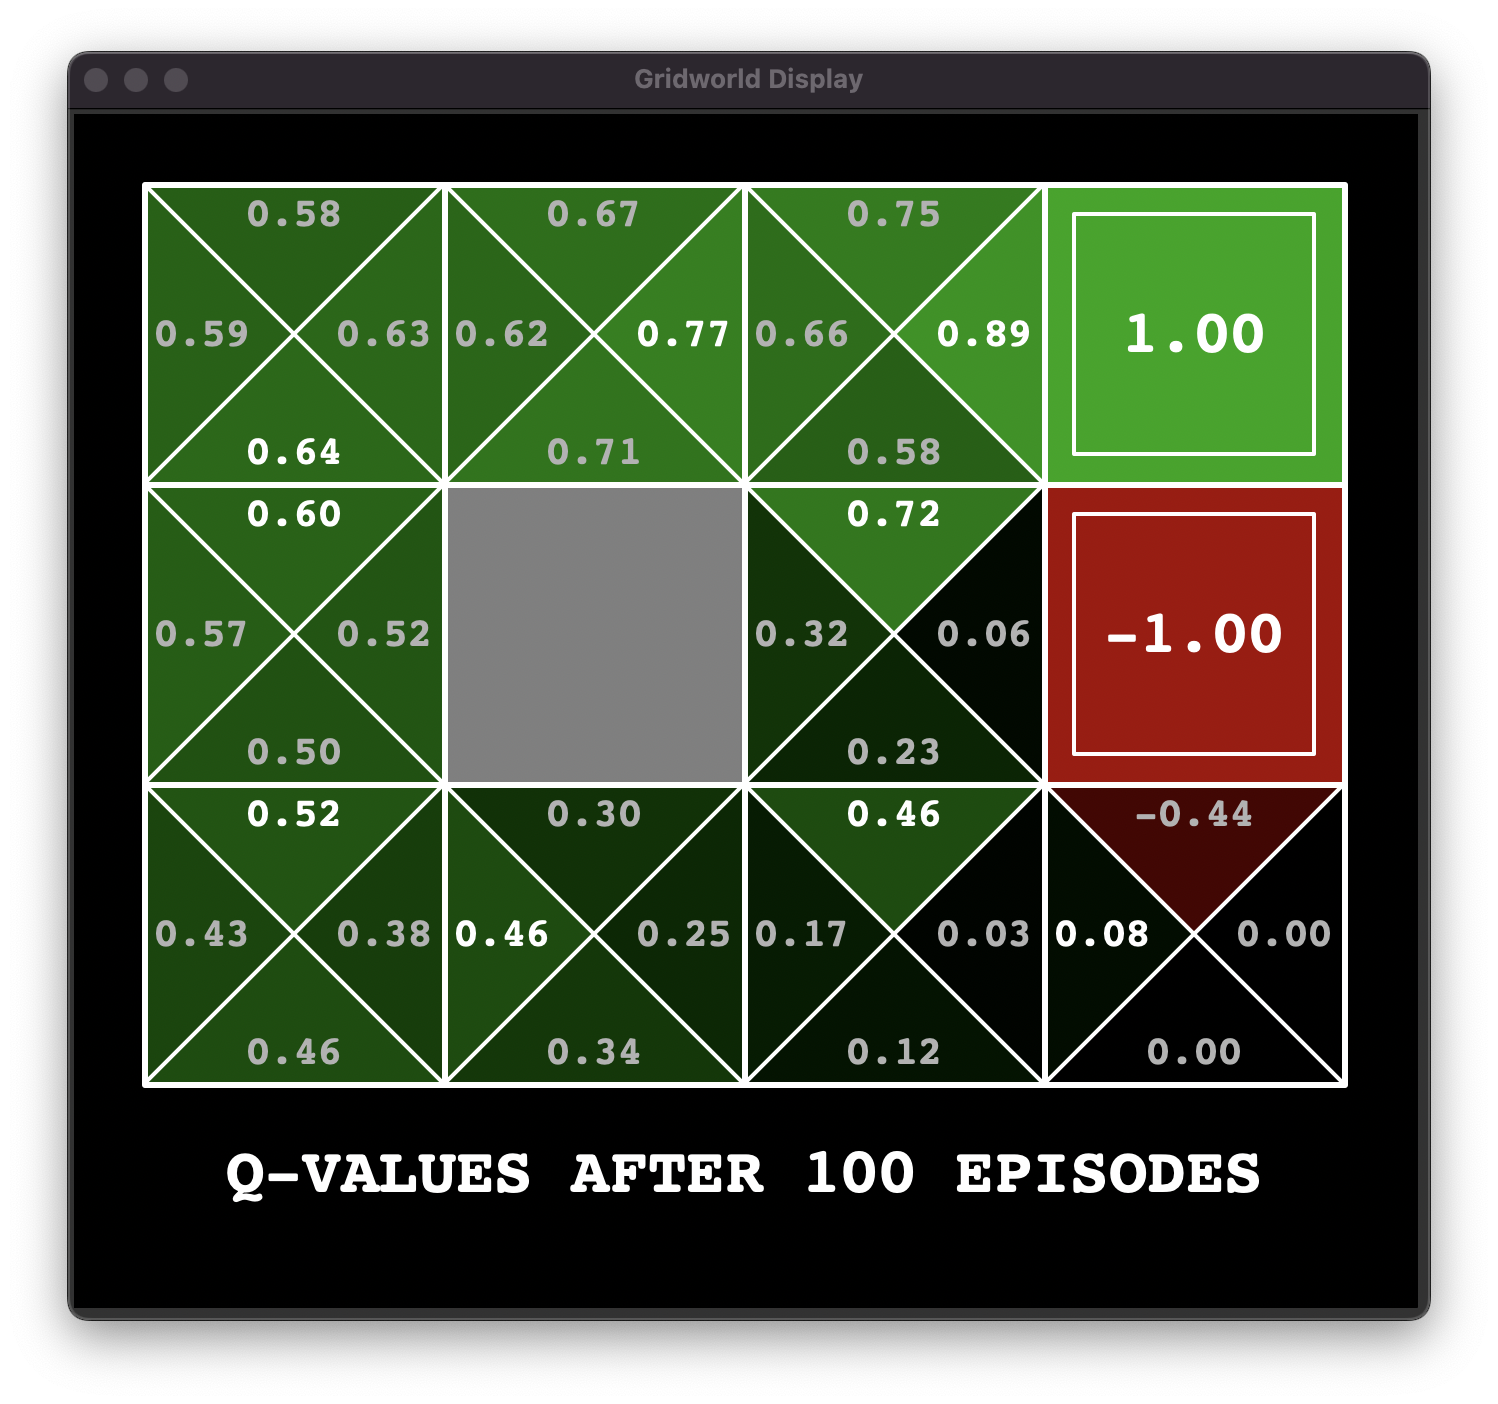
\includegraphics[width=0.5\textwidth]{images/qLearning-ex4.png}
  \end{center}
\caption{Q-Learning agent with episilon-greedy cut}
\end{table}

We can see that the agent sucessfully achieved the goal multiple times and changed the score of various squares of the grid. After seeing that it's functional we ran the crawler.py simulation and saw our agent evolving and reaching the end of the map, as seen bellow:

\begin{table}[ht!]
  \begin{center}
    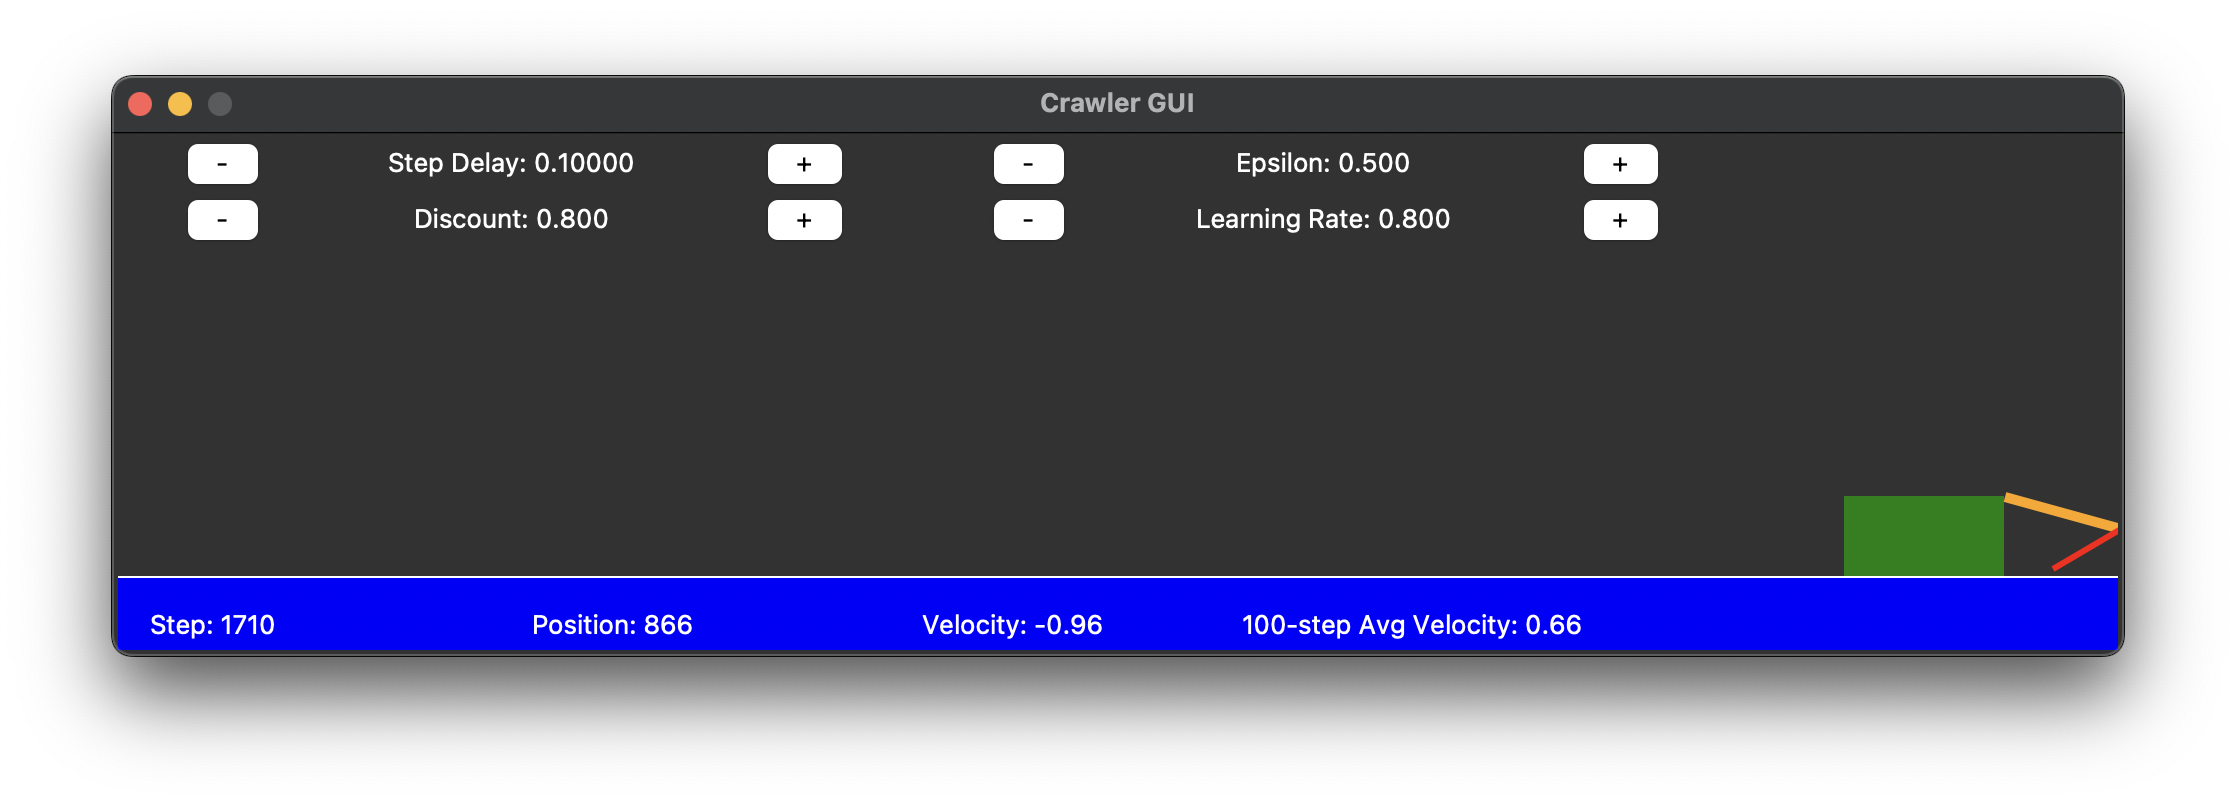
\includegraphics[width=1\textwidth]{images/crawler.png}
  \end{center}
\caption{Q-Learning agent in crawler.py simulation}
\end{table}

The final step for the Q-Learning agent was to apply it to the Pacman game, for this we ran the following command:

\definecolor{light-gray}{gray}{0.95}
\begin{lstlisting}[language=bash, frame=tlbr, framesep=6pt, backgroundcolor=\color{light-gray}]
  python3 pacman.py -p PacmanQAgent -x 2000 -n 2010 -l smallGrid
\end{lstlisting}

The first 2000 interations are used to train the agent and the last 10 are used to test it, the table bellow shows the reults of the training:

~\\
\begin{table}[!ht]
  \begin{center}
    \begin{tabular}{||c||c|c|c||}
      \hline
      Completed & Average Rewards over all training & Average Rewards for last 100 episodes & Time per episode\\
      \hline\hline
      100/2000 & -511.96 & -511.96 & 0.20s \\
      \hline\hline
      200/2000 & -512.18 & -512.41 & 0.25s \\
      \hline
      300/2000 & -488.55 & -441.29 & 0.25s \\
      \hline
      400/2000 & -452.35 & -343.74 & 0.31s \\
      \hline
      500/2000 & -423.72 & -309.20 & 0.31s \\
      \hline
      600/2000 & -391.24 & -228.81 & 0.3s \\
      \hline
      700/2000 & -378.26 & -300.38 & 0.32s \\
      \hline
      800/2000 & -366.19 & -281.69 & 0.33s \\
      \hline
      900/2000 & -341.96 & -148.20 & 0.31s \\
      \hline
      1000/2000 & -305.32 & 24.51 & 0.31s \\
      \hline
      1100/2000 & -271.73 & 64.11 & 0.32s \\
      \hline
      1200/2000 & -240.34 & 104.97 & 0.32s \\
      \hline
      1300/2000 & -202.12 & 256.52 & 0.31s \\
      \hline
      1400/2000 & -166.45 & 297.33 & 0.30s \\
      \hline
      1500/2000 & -140.89 & 216.90 & 0.30s \\
      \hline
      1600/2000 & -115.38 & 267.19 & 0.31s \\
      \hline
      1700/2000 & -91.70 & 287.31 & 0.31s \\
      \hline
      1800/2000 & -71.26 & 276.20 & 0.32s \\
      \hline
      1900/2000 & -55.58 & 226.59 & 0.31s \\
      \hline
      2000/2000 & -39.95 & 257.10 & 0.31s \\
      \hline
    \end{tabular}
    \caption{Training set Pacman}
    \label{tab:trainPac}
  \end{center}
\end{table}

After the training was done the Pacman proceded to testing generating the following results:

\begin{table}[!ht]
  \begin{center}
    \begin{tabular}{||c||c||}
      \hline
      Result & Scourse\\
      \hline\hline
      Win & 502 \\
      \hline\hline
      Win & 499 \\
      \hline
      Win & 503 \\
      \hline
      Win & 503 \\
      \hline
      Win & 495 \\
      \hline
      Win & 503 \\
      \hline
      Win & 499 \\
      \hline
      Win & 503 \\
      \hline
      Win & 503 \\
      \hline
      Win & 502 \\
      \hline
    \end{tabular}
    \caption{Test set Pacman}
    \label{tab:testPac}
  \end{center}
\end{table}

As seen in the table the Pacman achieved 100\% of the wins, which means that the agent was able to learn the game and play it perfectly.

\section{Approximate Q-Learning}

The last part of this report consists of an implementation of the Approximate Q-Learning algorithm, which is a variation of the Q-Learning algorithm that uses a function to approximate the Q-Values instead of a table.
The function used in this implementation is a linear combination of the features of the state, which are the position of the Pacman and the position of the ghosts.
The features are represented by a vector of 5 elements, the first 2 elements are the position of the Pacman and the last 3 elements are the position of the ghosts. 
The weights of the features are represented by a vector of 5 elements, the first 2 elements are the weights of the Pacman position and the last 3 elements are the weights of the ghosts position.
The Q-Value of a state is the dot product of the features vector and the weights vector.
The implementation of the Approximate Q-Learning algorithm is shown in the code bellow:

\begin{table} [ht!]
  \begin{lstlisting}[language=python, frame=tlbr, framesep=6pt, backgroundcolor=\color{light-gray}]
  def getQValue(self, state, action):
  """
    Should return Q(state,action) = w * featureVector
    where * is the dotProduct operator
  """
  Q = 0

  for i in self.featExtractor.getFeatures(state, action):
      Q += self.weights[i] * self.featExtractor.getFeatures(state, action)[i]
  
  return Q
  \end{lstlisting}
  \caption{getQValue function}
\end{table}

\begin{table} [ht!]
  \begin{lstlisting}[language=python, frame=tlbr, framesep=6pt, backgroundcolor=\color{light-gray}]
  def update(self, state, action, nextState, reward: float):
  """
     Should update your weights based on transition
  """
  difference = (reward + self.discount * \
    self.computeValueFromQValues(nextState)) - self.getQValue(state, action)
  for i in self.featExtractor.getFeatures(state, action):
      self.weights[i] += self.alpha * difference \ 
        * self.featExtractor.getFeatures(state, action)[i]

  return
  \end{lstlisting}
  \caption{update function}
\end{table}

\begin{table} [ht!]
  \begin{lstlisting}[language=python, frame=tlbr, framesep=6pt, backgroundcolor=\color{light-gray}]
  def final(self, state):
  """Called at the end of each game."""
  # call the super-class final method
  PacmanQAgent.final(self, state)

  # did we finish training?
  if self.episodesSoFar == self.numTraining:
      # you might want to print your weights here for debugging
      print(self.weights)
      pass
  \end{lstlisting}
  \caption{final function}
\end{table}

To test our agent we ran the following command, which simulates 10 games their results are shown in the table bellow:

\definecolor{light-gray}{gray}{0.95}
\begin{lstlisting}[language=bash, frame=tlbr, framesep=6pt, backgroundcolor=\color{light-gray}]
python3 pacman.py -p ApproximateQAgent -a \
extractor=SimpleExtractor -x 50 -n 60 -l mediumGrid
\end{lstlisting}

\begin{table}[!ht]
  \begin{center}
    \begin{tabular}{||c||c||}
      \hline
      Result & Scourse\\
      \hline\hline
      Win & 527 \\
      \hline\hline
      Win & 529 \\
      \hline
      Win & 525 \\
      \hline
      Win & 525 \\
      \hline
      Win & 527 \\
      \hline
      Win & 529 \\
      \hline
      Win & 527 \\
      \hline
      Win & 529 \\
      \hline
      Win & 527 \\
      \hline
      Win & 527 \\
      \hline
    \end{tabular}
    \caption{Test set Pacman}
    \label{tab:testPac}
  \end{center}
\end{table}

\pagebreak\pagebreak
\section{Conclusion}

By programming and implementing our own methods and agents, we were able to fully understand the functionings of the reinforcement learning and how it is an essential aspect in the domain of Artificial Inteligence.
On top of that we were able to understand the importance of the Markov Decision Process and how it is used in the reinforcement learning.

\end{document}